% This is LLNCS.DOC the documentation file of
% the LaTeX2e class from Springer-Verlag
% for Lecture Notes in Computer Science, version 2.4
\documentclass{article}

\usepackage{cite}
\usepackage{listings}
\usepackage{amssymb}
\usepackage{mathpartir}
\usepackage{amsmath}    
\usepackage{algpseudocode}
\usepackage{array}
\usepackage{xcolor}
\usepackage{fullpage}
\usepackage{graphicx}
\linespread{1.2}

\lstset{
    string=[s]{"}{"},
    stringstyle=\color{blue},
    comment=[l]{:},
    commentstyle=\color{black},
}


\begin{document}
\title{A Translation from the JSON Representation of CoCoSim Models to Lustre Programs}

\author{Baoluo Meng}


\maketitle

This is to document the translation process from the JSON representation of a CoCoSim model to its equivalent representation in Lustre.


\section{JSON Representation of CoCoSim Blocks}

CoCoSim supports a subset of the blocks provided by the Simulink toolset. Figure~\ref{basicmapping}~\ref{mapping2}~\ref{mapping3}~\ref{mapping4} summarize the supported blocks and the limitations on their semantics if it applies. 

A CoCoSim model is a visualization of a set of block declarations and their connectivities.
The CoCoSim intermediate compiler takes as input a Simulink model and translate it into a JSON representation storing blocks and connectivities information. 
The model information is stored as name -- value pairs in a JSON file. 
The name attribute specifies the name of the block, and the value stores the actual data about the block such as block handle, block connectivities and so on. 
Each block is uniquely identified by its block handle.
The ``BlockType" field specifies the type of a block. 
%For example, an inport block of a CoCoSim model has a ``BlockType" ``Inport".
The blocks connectivity information is stored in the ``PortConnectivity" field, where ``SrcBlock" stores the handles of incoming blocks, whereas ``DstBlock" stores the handles of destination blocks. 
The ``Origin\_path" is the full path to the block in the CoCoSim model.
The value of ``Ports" of inports or outports is the position index in the inputs or outputs. 

Figure~\ref{cocosimmodel} shows an overview of a CoCoSim model ``unsafe\_1\_PP" and Figure~\ref{jsoninport} shows a snippet of an overview its JSON representation. 
``In1" and ``In2" are the names of the inport blocks, ``Inport" is the type of block ``In1", and the handle which is the unique identifier for ``In1" is ``77.0003662109375". 
``Out1" is the outport of the block.
The data type of ``In1" is stored in the attribute ``Outport" of ``CompiledPortDataTypes", which is Boolean. 
Since ``In1" is an inport of top most node, it only has destination blocks. 
The handles of its destination blocks are store as values \{79.0003662109375, 92.0008544921875\} in ``DstBlock" of ``PortConnectivity". 
The ``Origin\_path" of ``In1" is ``unsafe\_1\_PP/In1".
``In1" has a ports value of 1, meaning it is the first input. 
Subsystem is a type of subsystem, which defines the relations among ``In1", ``In2", and ``Out1". 
Safety is an observer block that defines a property in terms of inputs and outputs of the subsystem block ``unsafe\_1\_PP". 
Safety\_term is a terminator block.

Figure~\ref{jsonsafety} shows a snippet of the observer block ``safety" in JSON, which is a type of subsystem block with the annotation type ``ensures".
It connects with ``SrcBlock" with handles \{77.0003662109375, 78.0003662109375, 920008544921875\}, which are the handles of inports ``In1" and ``In2" and outport ``Out1" of the calling node ``unsafe\_1\_PP",  and connects with ``DstBlock with handle ``91.000732421875", which is the handle of the terminator block. 

Figure~\ref{cocosimsafety} shows the CoCoSim model of the observer block ``Safety" and Figure~\ref{jsonsafetybody} shows the blocks definition of the observer block body in JSON, including 
three inports ``In1", ``In2", and ``Out1", an outport ``Safety", a logical operator ``AND", and a relational operator ``$>=$". 
Based on the connectivities defined in the port connectivity, ``Safety" connects with the source block logical operator ``AND", the logical operator ``AND" connects with the source blocks relational operator ``$>=$" and the inport block ``Out1", and the relational operator ``$>=$" connects
with the source block inports ``In1" and ``In2". 

\begin{figure}[h]
\begin{center}
    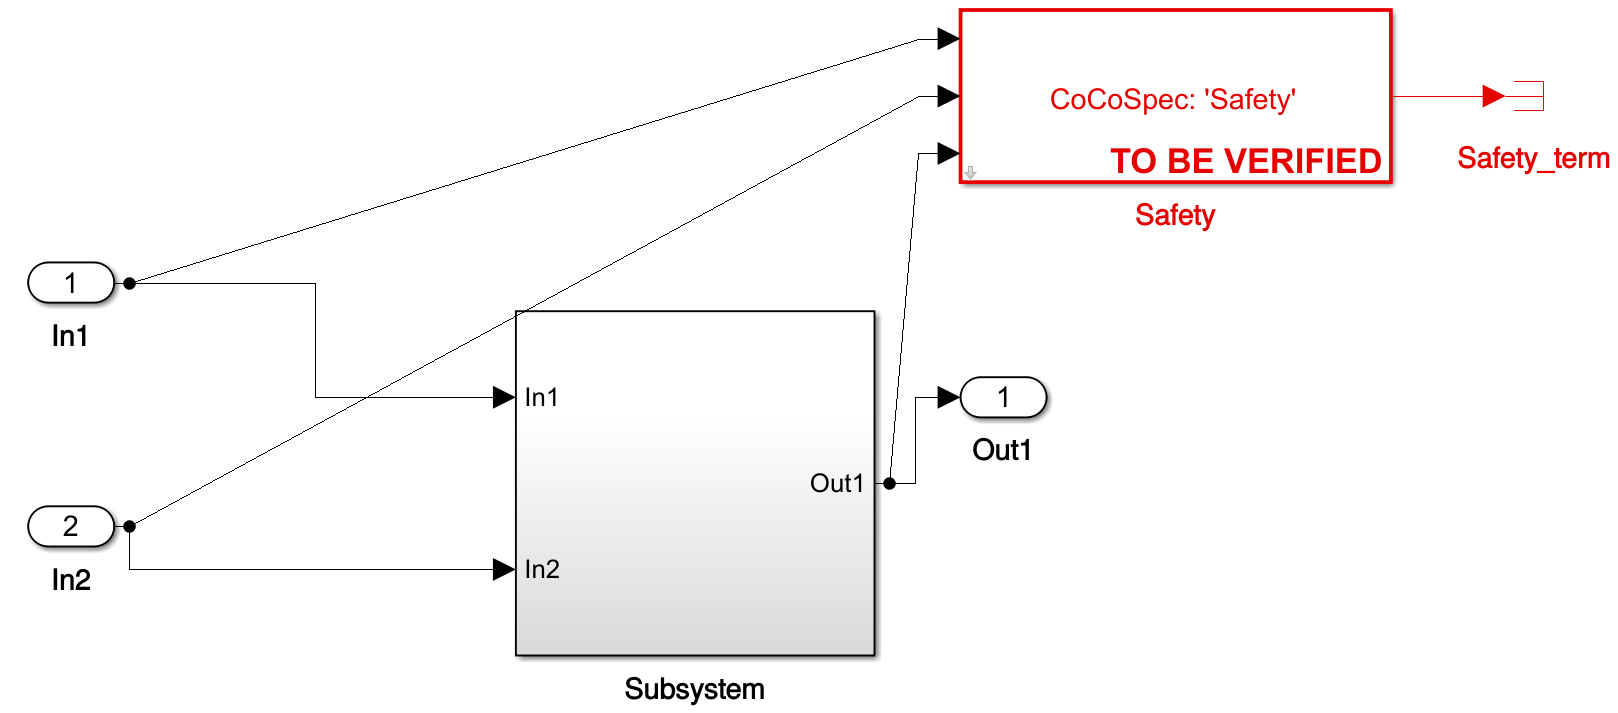
\includegraphics[scale=0.28]{figures/safety000}
\end{center}  
  \caption{A CoCoSim Model}
  \label{cocosimmodel}
\end{figure}

\begin{figure}[h]
\begin{center}
  \includegraphics[scale=0.5]{figures/in1}
\end{center}  
  \caption{A JSON snippet of the CoCoSim Model}
  \label{jsoninport}
\end{figure}

\begin{figure}[h]
\begin{center}
  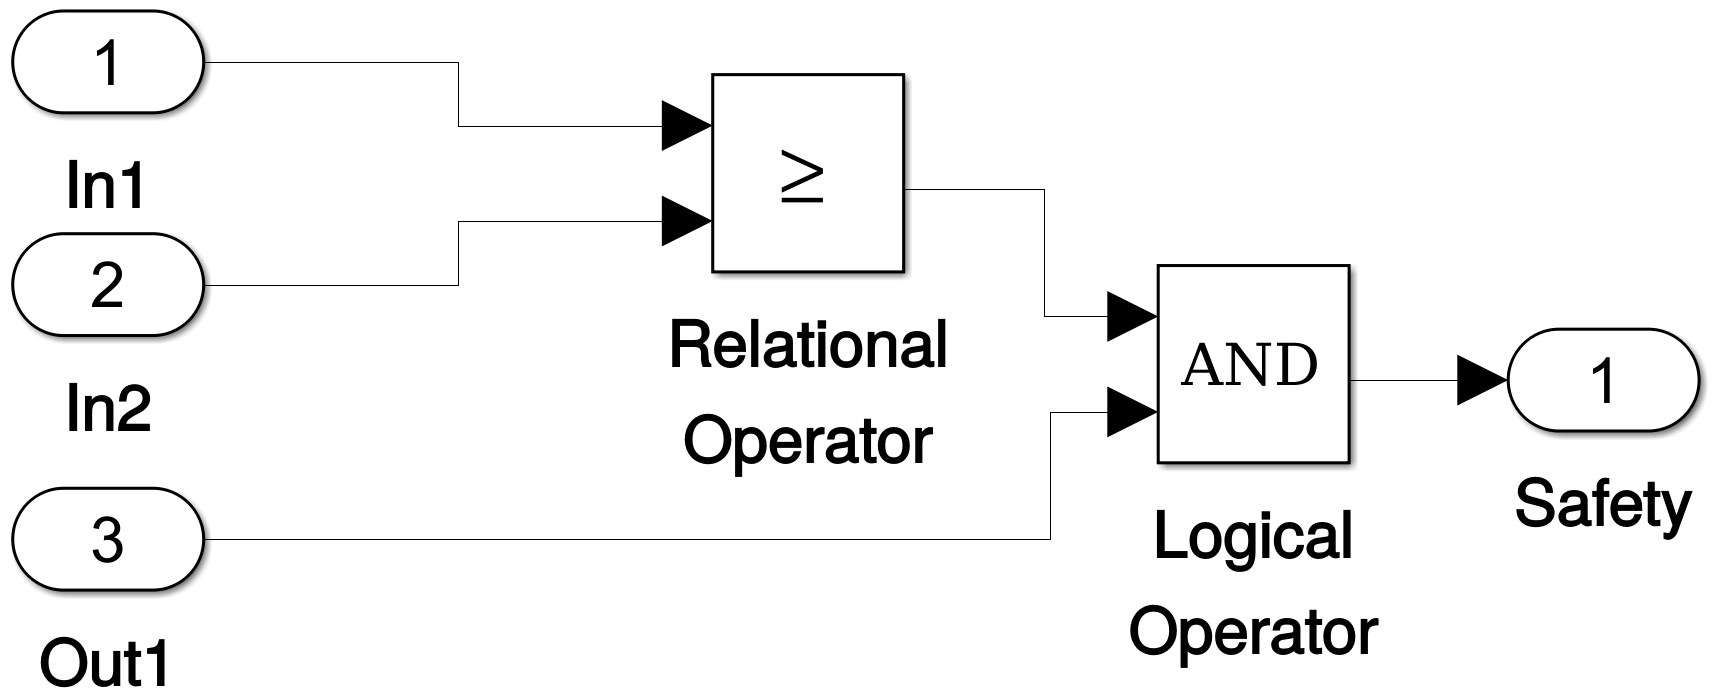
\includegraphics[scale=0.2]{figures/safety0}
\end{center}  
  \caption{A CoCoSim of the observer block safety}
  \label{cocosimsafety}
\end{figure}


\begin{figure}[h]
\begin{center}
  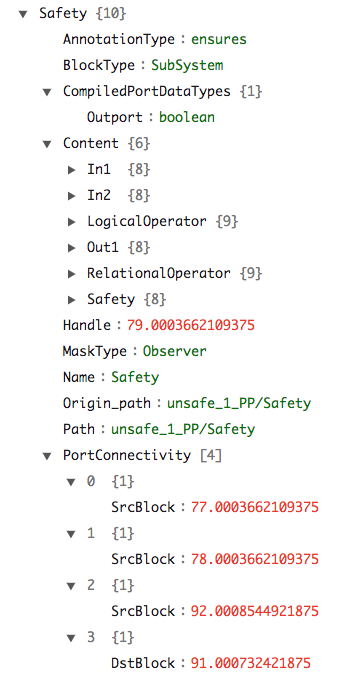
\includegraphics[scale=0.5]{figures/safety}
\end{center}  
  \caption{A JSON snippet of the observer block safety}
  \label{jsonsafety}
\end{figure}

\begin{figure}[h]
\begin{center}
  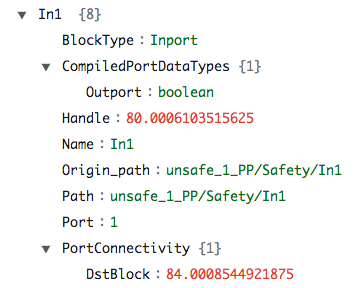
\includegraphics[scale=0.4]{figures/safety1}
    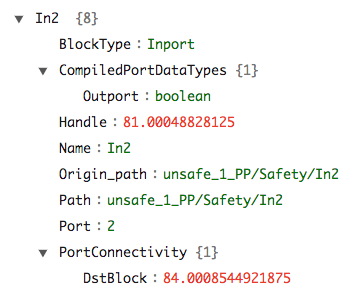
\includegraphics[scale=0.4]{figures/safety2}
  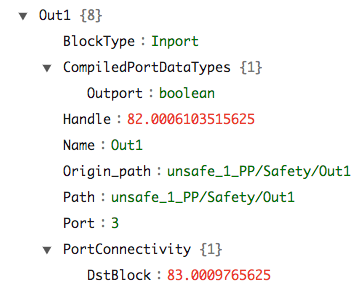
\includegraphics[scale=0.4]{figures/safety4}     
    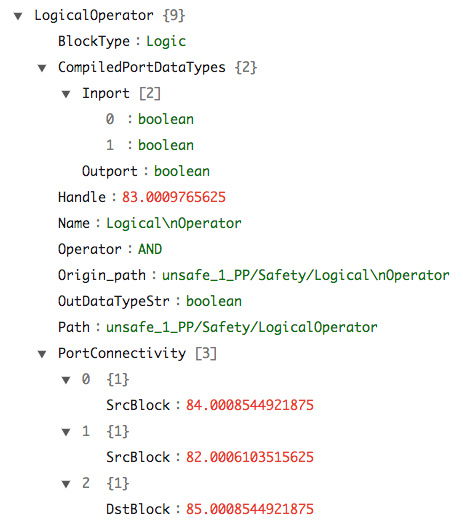
\includegraphics[scale=0.4]{figures/safety3}
    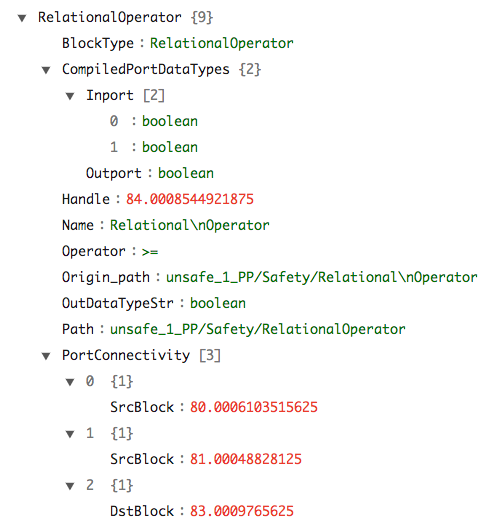
\includegraphics[scale=0.4]{figures/safety5}      
    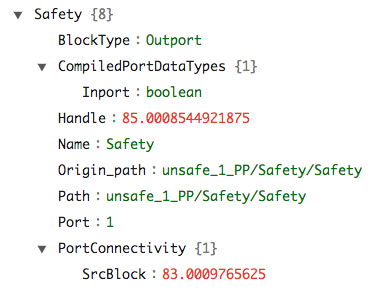
\includegraphics[scale=0.4]{figures/safety6}       
    
\end{center}  
  \caption{A JSON snippet of the body of the observer block safety}
  \label{jsonsafetybody}
\end{figure}

\subsection{A mapping from basic CoCoSim blocks to Lustre}

\begin{figure}[h]
\begin{center}
  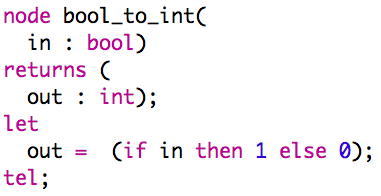
\includegraphics[scale=0.4]{figures/lus0}
  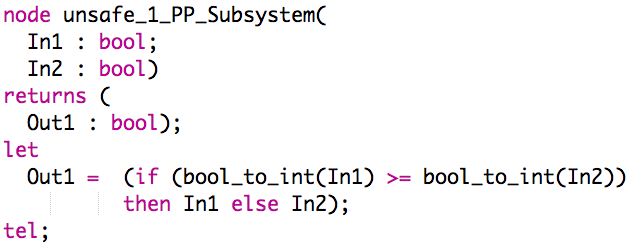
\includegraphics[scale=0.4]{figures/lus1}
  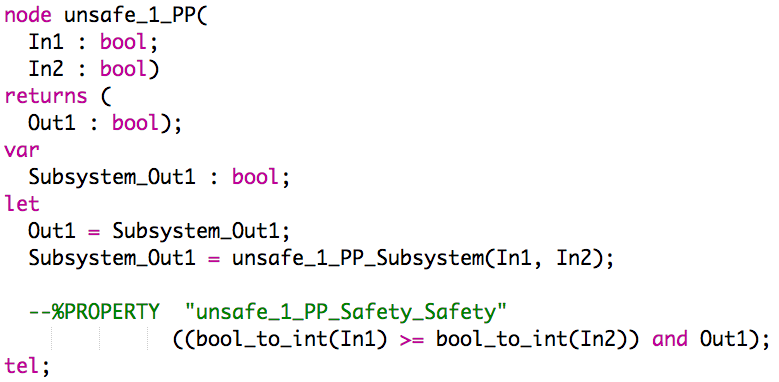
\includegraphics[scale=0.4]{figures/lus2}  
    
\end{center}  
  \caption{The translated Lustre programs for the CoCoSim model unsafe\_1\_PP}
  \label{lus}
\end{figure}

Figure~\ref{basicmapping} shows a mapping from basic CoCoSim blocks to their equivalent representations in Lustre.

\paragraph{Subsystem, Inport, and Outport} 
Subsystems create a hierarchical model comprising many layers. 
A subsystem is a set of blocks that you replace with a single \textsf{Subsystem} block. 
Subsystem normally consists of a set of inports and a set of outports, where outports are
defined by using inports and other blocks. 
In principle, almost all subsystems are translated into nodes in Lustre with inports being the 
inputs and outports being the outputs except for the observer subsystems and other minor blocks. 
The order of inputs and outputs are maintained during the translation. 
The hierarchical information about the model is translated into node calls.

An exception would be the observer node.
It will be inlined in the calling node as property statements instead of translating them 
as separate nodes.

\*

\indent \indent \indent \indent \textsf{-\ -\%PROPERTY ``property" property expression}

\*


\noindent The \textsf{property} is the output variable name and the expression is translated 
by substituting the input and output variables by concrete ones.

The translation is initiated by translating the outports backwardly. 
Each outport and its connected expressions are translated into an equation, where the outport is the output of the equation 
and the left hand side is the definition of the output.
They are translated recursively.
Figure ~\ref{lus} shows the translated Lustre programs corresponding to the CoCoSim model ``unsafe\_1\_PP".
Each expression is defined in terms of the following operators. 
We will describe the mappings of those operators in Lustre in the following paragraphs.

\paragraph{Subsystem} 
Subsystems are translated as node calls. 


\paragraph{Relational Operators} 
Relational operators greater than, less than, equal to, not equal to, greater 
than or equal to, and less than or equal to are translated into their counterparts 
($>, <, =, <>, >=, <=$) in Lustre.


\paragraph{Logical Operators} 
Logical operators AND, OR, NOT and XOR are translated into Lustre operators 
\textsf{and, or, not} and \textsf{xor}.
Other logical operators NAND, NOR, and NXOR are represented by using Lustre 
operators \textsf{not} and others.

\paragraph{Mathematical Operators} 
Mathematical operators sum, subtract, multiply, divide and mod are translated into 
\textsf{+}, \textsf{-}, \textsf{*}, \textsf{div} and \textsf{mod} respectively.
Operator Gain is translated into \textsf{*}. 
Operator Abs is translated into a node Abs. 
Operator Minmax is translated into a node Min or Max depending on the semantics of the subsystem. 
Operator CompareToZero/Constant is translated into a node CompareToZero/Constant.

\paragraph{Time Operators}
Operators Memory and UnitDelay are translated into the same time operator \textsf{pre} with the 
values of First and X0 as their initial conditions respectively.
Since Memory and UnitDelay may have the circular dependency issue, we introduce local variables for the 
portion of expression under \textsf{pre} to break the circular dependency if any. 

\begin{figure}[t]
\[
\begin{array}{l@{\qquad}llll}
 \text{constant} & c & := & 
true \mid false
 \\[0ex]
 \text{number} & n & := & 
 1 \cdots 9 (.1 \cdots 9)
 \\[0ex]
  \text{literal} & v & := & 
u n \mid n \mid c
 \\[0ex]
\text{unary expression} & e & := & 
-\ e \mid \sim e \mid \sim b \mid v
 \\[0ex]
 \text{binary expression} & b & := & 
e_1\ (>, <, >=, <=, ==, \sim=)\ e_2 
 \\[0ex]
\end{array}       
\]
\caption{The syntax for the conditional expresions}
\label{fig:grammar}
\end{figure}

\paragraph{Conditional Operators}
Operator SwitchCase is translated into \textsf{if $\cdots$ then $\cdots$ else if $\cdots$ then $\cdots$ }. 
For the IF operator, the conditional expressions are translated separately using the
expression parser \emph{ParBoiled} as the conditional expressions are in the string format. 
The expressions are defined by the syntax in Figure~\ref{fig:grammar}.

When parsing the expressions, the expression will be constructed as an abstract syntax tree. 
As we traverse the abstract syntax tree, the variables will be substituted by the concrete expressions
that are corresponding to.

\subsubsection{Types}

Types in CoCoSim models are loosely defined. 
They can be mixed compared, i.e., an integer can be compared to a Boolean.
However, Lustre language is strictly defined with types.
To be better handle types in CoCoSim models, we define six auxiliary functions
for converting typed expressions.
They are \textsf{bool\_to\_int, bool\_to\_real, int\_to\_bool, 
real\_to\_bool, real\_to\_int} and \textsf{int\_to\_real}. 

While translating expressions comparisons, if two expressions are compared, 
their types will be lifted to the highest type. For example, if a Boolean variable \textsf{a} 
is compared with an integer \textsf{b} for equality, \textsf{a} will be lifted to the integer 
type by calling the function \textsf{bool\_to\_int} and compared afterwards. 
If an expression is typed with Integer or Real and it is used as Boolean in the model,  it will be lowered 
to a Boolean by calling the function \textsf{int\_to\_bool} or \textsf{real\_to\_bool}.
 

\begin{figure}[t]
\centering
{
\begin{tabular}{lp{5cm}}
\hline
\textbf{CoCoSim} & \textbf{Lustre}  \\
\hline
SubSystem & 
Node
\\
Inport &
Input
\\
Outport &
Output
\\
Gain &
Multiply input by constant ($\times$)
\\

Abs (in) &
Use library node Abs(in)
\\

AND, OR, NAND, NOR, XOR, NXOR, NOT
&
and, or, not and, not or, xor, not xor, not
\\

Minmax &
{Dynamically create minimum or maximum nodes}
\\

SwitchCase &
{if ... then ... else if ... }
\\

Sum &
$+$
\\

Saturate &
The Saturation block imposes upper and lower limits on an input signal ($<=, <$)
\\

RelationalOperator &
$==, <>, <, <=, >, >=$
\\

UnitDelay &
pre
\\

If &
if ... then ... else ...
\\

Memory &
Output input from previous time step (pre)
\\

Compare To Zero/Constant  &
$==, <>, <, <=, >, >=$
\\

Math(mod, square, substract, divide, negative) &
mod, $\times, -, /, - $, 
\\

Constant &
constant
\\

\hline
\end{tabular}
}
\caption{A mapping from basic CocoSim blocks to Lustre constructs}
\label{basicmapping}
\end{figure}


\subsection{The Translation of CoCoSim contracts}
The Kind 2 contracts are added as additional features for modeling CoCoSim models.
They are encapsulated in \textsf{Subsystem} blocks and are accessible by using customized 
blocks.
To distinguish the node type, we use the ``ContractBlockType" to indicate whether a block 
is an \textsf{assume}, \textsf{guarantee}, \textsf{mode}, \textsf{requires}, or \textsf{ensures} block.
The contract always returns a Boolean typed variable \textsf{valid}.
The translation ignores the variable \textsf{valid} and construct the signature 
of the contract by looking at the signature of the calling node.
The translation process of expressions is the same as described above. 

\subsection{The Translation Algorithm}

We describe here the translation algorithm for the JSON model. 


\begin{figure}
\begin{algorithmic}
\Function{\textbf{translate}}{Node rootNode}
\Return{(LustreProgram P)}
\State \textbf{let} subsystems = \{S $\mid$ S is a subsystem block $\land$ S $\in$ rootNode.fields\} \textbf{in}
\State \textbf{for} subsystem : subsystems
\State {\ \ \ \ } \textbf{let} ast = \textbf{translateSubsystem}(subsystem) \textbf{in}
\State {\ \ \ \ } \textbf{if}  ast \textbf{instanceof} LustreNode \textbf{then}
\State {\ \ \ \ \ \ \ \ } P.addNode(ast)
\State {\ \ \ \ } \textbf{else}
\State {\ \ \ \ \ \ \ \ } P.addContract(ast)
\EndFunction
\end{algorithmic}

\begin{algorithmic}
\Function{\textbf{translateSubsystem}}{Node subsystem}
\Return{(LustreAst ast)}

\State \textbf{let} inputs = \{\} \textbf{in}
\State \textbf{let} props = \{\} \textbf{in}
\State \textbf{let} outputs = \{\} \textbf{in}
\State \textbf{let} contract = \{\} \textbf{in}
\State \textbf{let} hdlToBlk = \{\} \textbf{in}
\State \textbf{let} blkToSrcHdls = \{subsystem $\mapsto$ subsystem.getSrcHdls()\} \textbf{in}
\State \textbf{let} blkToDstHdls = \{subsystem $\mapsto$ subsystem.getDstHdls()\} \textbf{in}
\State \textbf{for} cntBlk : subsystem.contentFields()
\State {\ \ \ \ }  blkToSrcHdls $\leftarrow$ \{cntBlk $\mapsto$ cntBlk.getSrcHdls()\};
\State {\ \ \ \ }  blkToDstHdls $\leftarrow$ \{cntBlk $\mapsto$ cntBlk.getDstHdls()\};
\State {\ \ \ \ } hdlToBlk $\leftarrow$ \{cntBlk.getHdl() $\mapsto$ cntBlk\};
\State {\ \ \ \ } \textbf{match}  cntBlk.getBlkType() \textbf{with}
\State {\ \ \ \ } $\mid$ PROP $\rightarrow$ props $\leftarrow$ cntBlk
\State {\ \ \ \ } $\mid$ INPORT $\rightarrow$ inputs $\leftarrow$ \{\textbf{LustreVar}(cntBlk), contBlk\}
\State {\ \ \ \ } $\mid$ OUTPORT $\rightarrow$ outputs $\leftarrow$ \{\textbf{LustreVar}(cntBlk), contBlk\}
\State {\ \ \ \ } $\mid$ CONTRACT $\rightarrow$ contracts $\leftarrow$ cntBlk
\State \textbf{if} subsystem.isContract() \textbf{then}
\State {\ \ \ \ } \textbf{translateForContract}(subsystem, hdlToBlk, blkToSrcHdls, blkToDstHdls);
\State \textbf{else}
\State {\ \ \ \ } \textbf{translateForLusNode}(subsystem, inputs, outputs, props, contracts, hdlToBlk, blkToSrcHdls, 
\State {\ \ \ \ \ \ \ \ \ \ \ \ \ \ \ \ \ \ \ \ \ \ \ \ \ \ \ \ \ \ \ \ \ \ \ \ } blkToDstHdls);
\EndFunction
\end{algorithmic}
\caption{The translation algorithm}
\end{figure}


\begin{figure}
\begin{algorithmic}
\Function{\textbf{translateForLusNode}}{Node subsystem, Map inputs, Map outputs, List props, List contracts, Map hdlToBlk, Map blkToSrcHdls, Map blkToDstHdls}
\Return{(LustreAst ast)}
\State \textbf{let} equations = \{\} in
\State \textbf{for} (var, outputBlk) : outputs.values()
\State {\ \ \ \ } equations $\leftarrow$ \textbf{LusEquation}(var, \textbf{translateBlock}(outputBlk));

\EndFunction
\end{algorithmic}
\caption{The translateForLusNode algorithm}
\end{figure}

\begin{figure}
\begin{algorithmic}
\Function{\textbf{translateBlock}}{Node blk, Map hdlToBlk, Map blkToSrcHdls, Map blkToDstHdls}
\\
\Return{(LustreAst ast)}
\State \textbf{let} inExprs = \{\} \textbf{in}
\State \textbf{let} blkType = blk.getBlkType() \textbf{in}
\State \textbf{let} inHdls = blkToSrcHdl.get(blk) \textbf{in}
\State \textbf{for} inHdl: inHdls
\State {\ \ \ \ } inExprs $\leftarrow$ \textbf{translateBlock}(hdlToBlk.get(inHdl), hdlToBlk, blkToSrcHdls, blkToDstHdls);
\State \textbf{match} blkType \textbf{with}
\State $\mid$ NOT $\rightarrow$ \textbf{UnaryExpr}(NOT, inExprs[0]);
\State $\mid$ AND $\rightarrow$ \textbf{BinaryExpr}(AND, inExprs);
\State $\mid$ OR $\rightarrow$ \textbf{BinaryExpr}(OR, inExprs);
\State $\mid$ XOR $\rightarrow$ \textbf{BinaryExpr}(XOR, inExprs);
\State $\mid$ NAND $\rightarrow$ \textbf{BinaryExpr}(NAND, inExprs);
\State $\mid$ NOR $\rightarrow$ \textbf{BinaryExpr}(NOR, inExprs);
\State $\mid$ NXOR $\rightarrow$ \textbf{BinaryExpr}(NXOR, inExprs);
\State $\mid$ SUM $\rightarrow$ \textbf{BinaryExpr}(SUM, inExprs);
\State $\mid$ MOD $\rightarrow$ \textbf{BinaryExpr}(inExprs[0], MOD, inExprs[1]);
\State $\mid$ EQ $\rightarrow$ \textbf{BinaryExpr}(inExprs[0], EQ, inExprs[1]);
\State $\mid$ NEQ $\rightarrow$ \textbf{BinaryExpr}(inExprs[0], NEQ, inExprs[1]);
\State $\mid$ GTE $\rightarrow$ \textbf{BinaryExpr}(inExprs[0], GTE, inExprs[1]);
\State $\mid$ LTE $\rightarrow$ \textbf{BinaryExpr}(inExprs[0], LTE, inExprs[1]);
\State $\mid$ GT $\rightarrow$ \textbf{BinaryExpr}(inExprs[0], GT, inExprs[1]);
\State $\mid$ LT $\rightarrow$ \textbf{BinaryExpr}(inExprs[0], LT, inExprs[1]);

\State $\mid$ UNARYMINUS $\rightarrow$ \textbf{UnaryExpr}(UNARYMINUS, inExprs[1]);
\State $\mid$ COMPARETOCONST $\rightarrow$ \textbf{BinaryExpr}(inExprs[0], OP, \textbf{Constant});
\State $\mid$ COMPARETOZERO $\rightarrow$ \textbf{BinaryExpr}(inExprs[0], OP, \textbf{Zero});
\State $\mid$ SUBSYSTEM $\rightarrow$ \textbf{getBlkName}(blk)(inExprs);
\State $\mid$ INPORT $\rightarrow$ \textbf{Constant}(\textbf{getBlkName}(blk));
\State $\mid$ CONSTANT $\rightarrow$ \textbf{Constant}(\textbf{getValue}(blk));
\State $\mid$ PRODUCT $\rightarrow$ \textbf{Expr}(PRODUCT, inExprs);
\State $\mid$ ARROW $\rightarrow$ \textbf{BinaryExpr}(inExprs[0], ARROW, \textbf{Zero});
\State $\mid$ MEMORY/UNITDELAY $\rightarrow$ \textbf{BinaryExpr}(init, PRE, inExprs[0]);
\EndFunction
\end{algorithmic}
\caption{The translation algorithm}
\end{figure}

\subsection{Semantics of complex CoCoSim blocks}

\begin{figure}[t]
\centering
{
\begin{tabular}{lp{5cm}}
\hline
\textbf{CocoSim} & \textbf{Semantics}  \\
\hline
Switch &
{Switch output between first input and third input based on value of second input}

\\
Mux &
Combine several input signals into vector
\\


Demux &
Extract and output elements of vector signal
\\

Trigonometry &
Not Support
\\

DiscreteStateSpace &
Gain
\\

Goto/From &
Pass block input to From blocks/Accept input from Goto block
\\

Bias &
The Bias block adds a bias, or offset, to the input signal ($Y = U + bias$), where U is the block input and Y is the output.
\\

Concatenate &
?? Concatenate input signals of same data type to create contiguous output signal
\\

MultiPortSwitch &
Choose between multiple block inputs. Can be translated to if-then-else
\\

Reshape &
Change dimensionality of signal
\\

DiscreteIntegrator &
Perform discrete-time integration or accumulation of signal
\\

Saturation Dynamic &
The Saturation Dynamic block bounds the range of an input signal to upper and lower saturation values. The input below the lower limit is set to the lower limit. The input above the upper limit is set to the upper limit.
\\

Zero Pole &
The Zero-Pole block models a system that you define with the zeros, poles, and gain of a Laplace-domain transfer function. 
\\

\hline
\end{tabular}
}
\caption{A mapping from CocoSim to Lustre}
\label{mapping2}
\end{figure}



\begin{figure}[t]
\centering
%\scriptsize
{
\begin{tabular}{lp{6cm}}
\hline
\textbf{CocoSim} & \textbf{Semantics}  \\
\hline

Detect Change &
The Detect Change block determines if an input does not equal its previous value.
\\

Detect Increase &
The Detect Increase block determines if an input is strictly greater than its previous value.
\\

Detect Decrease &
The Detect Decrease block determines if an input is strictly less than its previous value.
\\

Detect Rise Positive &
The Detect Rise Positive block determines if the input is strictly positive, and its previous value was nonpositive.
\\

Detect Rise Nonnegative &
The Detect Rise Nonnegative block determines if the input is greater than or equal to zero, and its previous value was less than zero.
\\

Detect Fall Negative &
The Detect Fall Negative block determines if the input is less than zero, and its previous value was greater than or equal to zero.
\\

Detect Fall Nonpositive &
The Detect Fall Nonpositive block determines if the input is less than or equal to zero, and its previous value was greater than zero.
\\


Fcn &
Apply specified expression to input
\\

Matlab function &
Gain
\\

ActionPort &
Implement Action subsystems used in if and switch control flow statements
\\

TriggerPort &
Adding a Trigger block to a model or subsystem allows an external signal to trigger its execution.
\\

EnablePort &
Gain
\\

\hline
\end{tabular}
}
\caption{A mapping from CocoSim to Lustre}
\label{mapping3}
\end{figure}


\begin{figure}[t]
\centering
%\scriptsize
{
\begin{tabular}{lp{6cm}}
\hline
\textbf{CocoSim} & \textbf{Semantics}  \\
\hline

Assignment &
Gain
\\

Selector &
Select input elements from vector, matrix, or multidimensional signal
\\

DataTypeConversion &
Convert input signal to specified data type
\\

ForIterator &
Repeatedly execute contents of subsystem at current time step until iteration variable exceeds specified iteration limit
\\

DiscreteFilter &
Model Infinite Impulse Response (IIR) filters
\\

Polyval &
The Polynomial Evaluation block applies a polynomial function to the real or complex input at the In port.
\\

LookupNDDirect &
Index into N-dimensional table to retrieve element, column, or 2-D matrix
\\

SignalSpecification &
Specify desired dimensions, sample time, data type, numeric type, and other attributes of signal
\\

BusCreator &
Create signal bus
\\

BusSelector &
Select signals from incoming bus
\\

BusAssignment &
Replace specified bus elements
\\

Bitwise (AND, OR, NAND, NOR, XOR, NOT) &
AND, OR, NAND, NOR, XOR, NOT
\\

DotProduct &
Generate dot product of two vectors
\\

Signum &
Y = sign(x) returns an array Y the same size as x according to some rules.
\\

CrossProduct &
Calculate cross product of two vectors
\\

Merge &
Combine multiple signals into single signal
\\

\hline
\end{tabular}
}
\caption{A mapping from CocoSim to Lustre}
\label{mapping4}
\end{figure}

\end{document}
















